% Results and Analysis – tables and figures first

\subsection{Single-Model Baselines}

% Auto-generated tables
\begin{table}[h]
  \centering
  \caption{Single-model performance on combined validation.}\label{tab:single_models_auto}
  {\small
  \begin{tabular}{lcccccc}
  \toprule
  Model & AUC & F1 & Acc & Prec & Rec & FNR \\ \midrule
  MobileNetV4 (Stage~1; routing-only) & 0.9936 & N/A & N/A & N/A & N/A & N/A \\
  EfficientNetV2 (Stage~2, b3) & 0.9633 & 0.8930 & 0.8946 & 0.8806 & 0.9057 & 0.0943 \\ 
  \bottomrule
  \end{tabular}}
\end{table}

\begin{table}[h]
  \centering
  \caption{Best cascade configurations.}\label{tab:cascade_best_auto}
  {\small
  \begin{tabular}{cccccc}
  \toprule
 Low & High & AUC & F1 & FNR & Escalation \\ \midrule
  0.05 & 0.55 & 0.9941 & 0.9654 & 0.0060 & 0.0116 \\ 
  0.03 & 0.55 & 0.9941 & 0.9644 & 0.0054 & 0.0150 \\ 
  \bottomrule
  \end{tabular}}
\end{table}

\begin{table}[h]
  \centering
  \caption{Deepfake-Eval-2024 (calibrated)}\label{tab:deepeval_calibrated}
  {\small
  \begin{tabular}{lccccc}
  \toprule
 Split & Acc & F1 & FNR & FPR & Stage2 Rate \\ \midrule
  test & 0.4995 & 0.2796 & 0.7901 & 0.2513 & 0.5226 \\ 
  val & 0.5804 & 0.2996 & 0.7288 & 0.2667 & 0.5108 \\ 
  \bottomrule
  \end{tabular}}
\end{table}

\begin{table}[h]
  \centering
  \caption{Deepfake-Eval-2024 (stage2only)}\label{tab:deepeval_stage2only}
  {\small
  \begin{tabular}{lccccc}
  \toprule
 Split & Acc & F1 & FNR & FPR & Stage2 Rate \\ \midrule
  test & 0.4647 & 0.5962 & 0.1456 & 0.8706 & 0.9891 \\ 
  val & 0.3273 & 0.4460 & 0.1817 & 0.9155 & 0.9751 \\ 
  \bottomrule
  \end{tabular}}
\end{table}

% Stage 1 per-dataset evaluation (calibrated)
\begin{table}[h]
  \centering
  \caption{Stage~1 per-dataset evaluation (calibrated).}\label{tab:stage1_per_dataset}
  {\small
  \begin{tabular}{lcccccc}\toprule
  Dataset & AUC & F1 & Acc & Prec & Rec & FNR \\ \midrule
  FaceForensics++ & 0.9683 & 0.9171 & 0.9138 & 0.8905 & 0.9453 & 0.0547 \\
  CelebDF-v2 & 0.9982 & 0.9771 & 0.9769 & 0.9611 & 0.9936 & 0.0064 \\
  DFDC & 0.9931 & 0.9546 & 0.9543 & 0.9512 & 0.9580 & 0.0420 \\
  DeeperForensics\,1.0 & 1.0000 & 0.9975 & 0.9976 & 1.0000 & 0.9951 & 0.0049 \\ 
  \midrule
  Macro Avg & 0.9899 & 0.9616 & 0.9607 & 0.9507 & 0.9730 & 0.0270 \\ 
  Micro Avg & 0.9934 & 0.9700 & 0.9695 & 0.9658 & 0.9744 & 0.0256 \\ 
  \bottomrule
  \end{tabular}}
\end{table}

% Stage 2 per-dataset evaluation
% NOTE: values taken from outputs/stage3/history/run_20251029_043420/per_dataset_evaluation.json
\begin{table}[h]
  \centering
  \caption{Stage~2 EfficientNetV2-B3 per-dataset evaluation at threshold 0.70 (combined validation).}
  \label{tab:stage2_per_dataset}
  {\small
  \begin{tabular}{lcccccc}\toprule
  Dataset & AUC & F1 & Acc & Prec & Rec & FNR \\ \midrule
  CelebDF-v2 & 0.7718 & 0.6751 & 0.7035 & 0.7438 & 0.6180 & 0.3820 \\
  FaceForensics++ & 0.8009 & 0.5897 & 0.6898 & 0.8160 & 0.4616 & 0.5384 \\
  DeeperForensics\,1.0 & 0.8576 & 0.4942 & 0.6817 & 0.9792 & 0.3305 & 0.6695 \\
  DFDC & 0.8968 & 0.8187 & 0.8144 & 0.8015 & 0.8366 & 0.1634 \\
  \bottomrule
  \end{tabular}}
\end{table}

\noindent The auto\hyp generated tables first summarise single\hyp model performance for Stage~1 (MobileNetV4) and the strongest Stage~2 expert on the combined validation split (Table~\ref{tab:single_models_auto}), and then provide per\hyp dataset breakdowns for both stages (Tables~\ref{tab:stage1_per_dataset} and~\ref{tab:stage2_per_dataset}). Across the combined validation manifest, the EfficientNetV2 expert attains higher AUC and F1 than the lightweight Stage~1 filter (AUC~\num{0.9633}, F1~\num{0.8930}, FNR~\num{0.0943}), but at a higher per\hyp sample cost. For Stage~1, datasets with more controlled acquisition conditions (e.g., CelebDF\,v2, FaceForensics++) achieve very high absolute performance, whereas more heterogeneous sources (e.g., DFDC, DeeperForensics) remain more challenging. The corresponding Stage~2 results, computed from the same cached logits at a fixed threshold (0.70), show a similar pattern with different operating points, motivating the cascaded design in which Stage~1 handles easy cases cheaply and escalates ambiguous inputs to the stronger expert, and Stage~4 tunes thresholds explicitly rather than relying on a single global cut\hyp off.

\noindent To make the trade\hyp offs between the two stages more explicit, Table~\ref{tab:stage1_stage2_compare} contrasts their combined\hyp validation performance. Stage~1 offers slightly higher AUC but does not by itself achieve the very low FNR that the tuned cascade can reach; Stage~2 provides stronger calibrated probabilities and serves as the high\hyp accuracy expert within the cascade.

\begin{table}[h]
  \centering
  \caption{Stage~1 vs.\ Stage~2 performance on the combined validation split. Stage~1 is used as a fast filter within the cascade; Stage~2 serves as the high-accuracy expert.}
  \label{tab:stage1_stage2_compare}
  {\small
  \begin{tabular}{lccc}
    \toprule
    Model & AUC & F1 & FNR \\
    \midrule
    Stage~1 MobileNetV4 filter & 0.9936 & N/A & N/A \\
    Stage~2 EfficientNetV2-B3 expert & 0.9633 & 0.8930 & 0.0943 \\
    \bottomrule
  \end{tabular}}
\end{table}

\noindent Note on GenConViT: We explored a GenConViT expert but, under our configuration and timeline, observed limited and inconsistent gains over the strongest single expert (EfficientNetV2). Primary single-model lines therefore reflect EfficientNetV2; GenConViT remains available as an optional expert and for meta-model fusion (see Method/Appendix).
% Intentionally kept minimal; device-side baselines will be added with on-device measurements.

\begin{figure}[h]
  \centering
  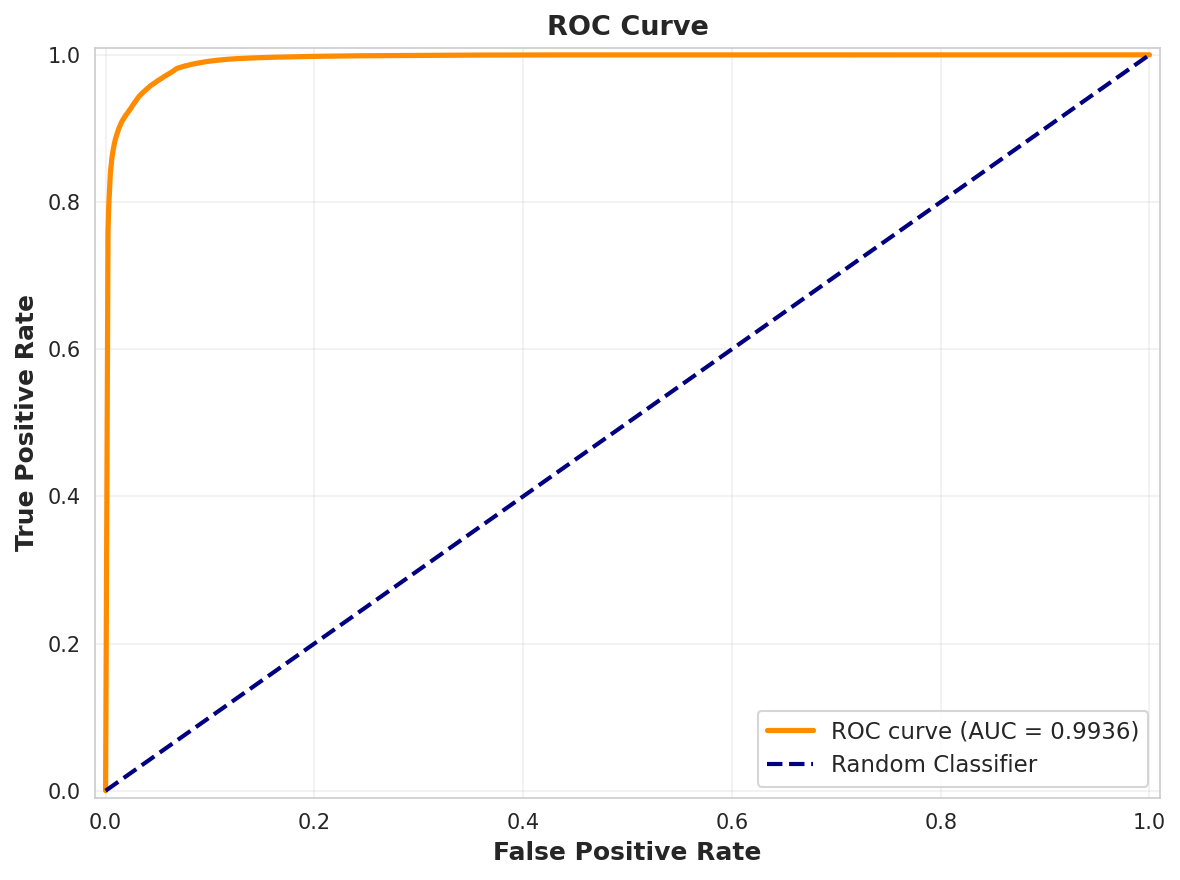
\includegraphics[width=.45\textwidth]{figures/outputs_stage1_run_20251023_034316_01_roc_curve.png}\hfill
  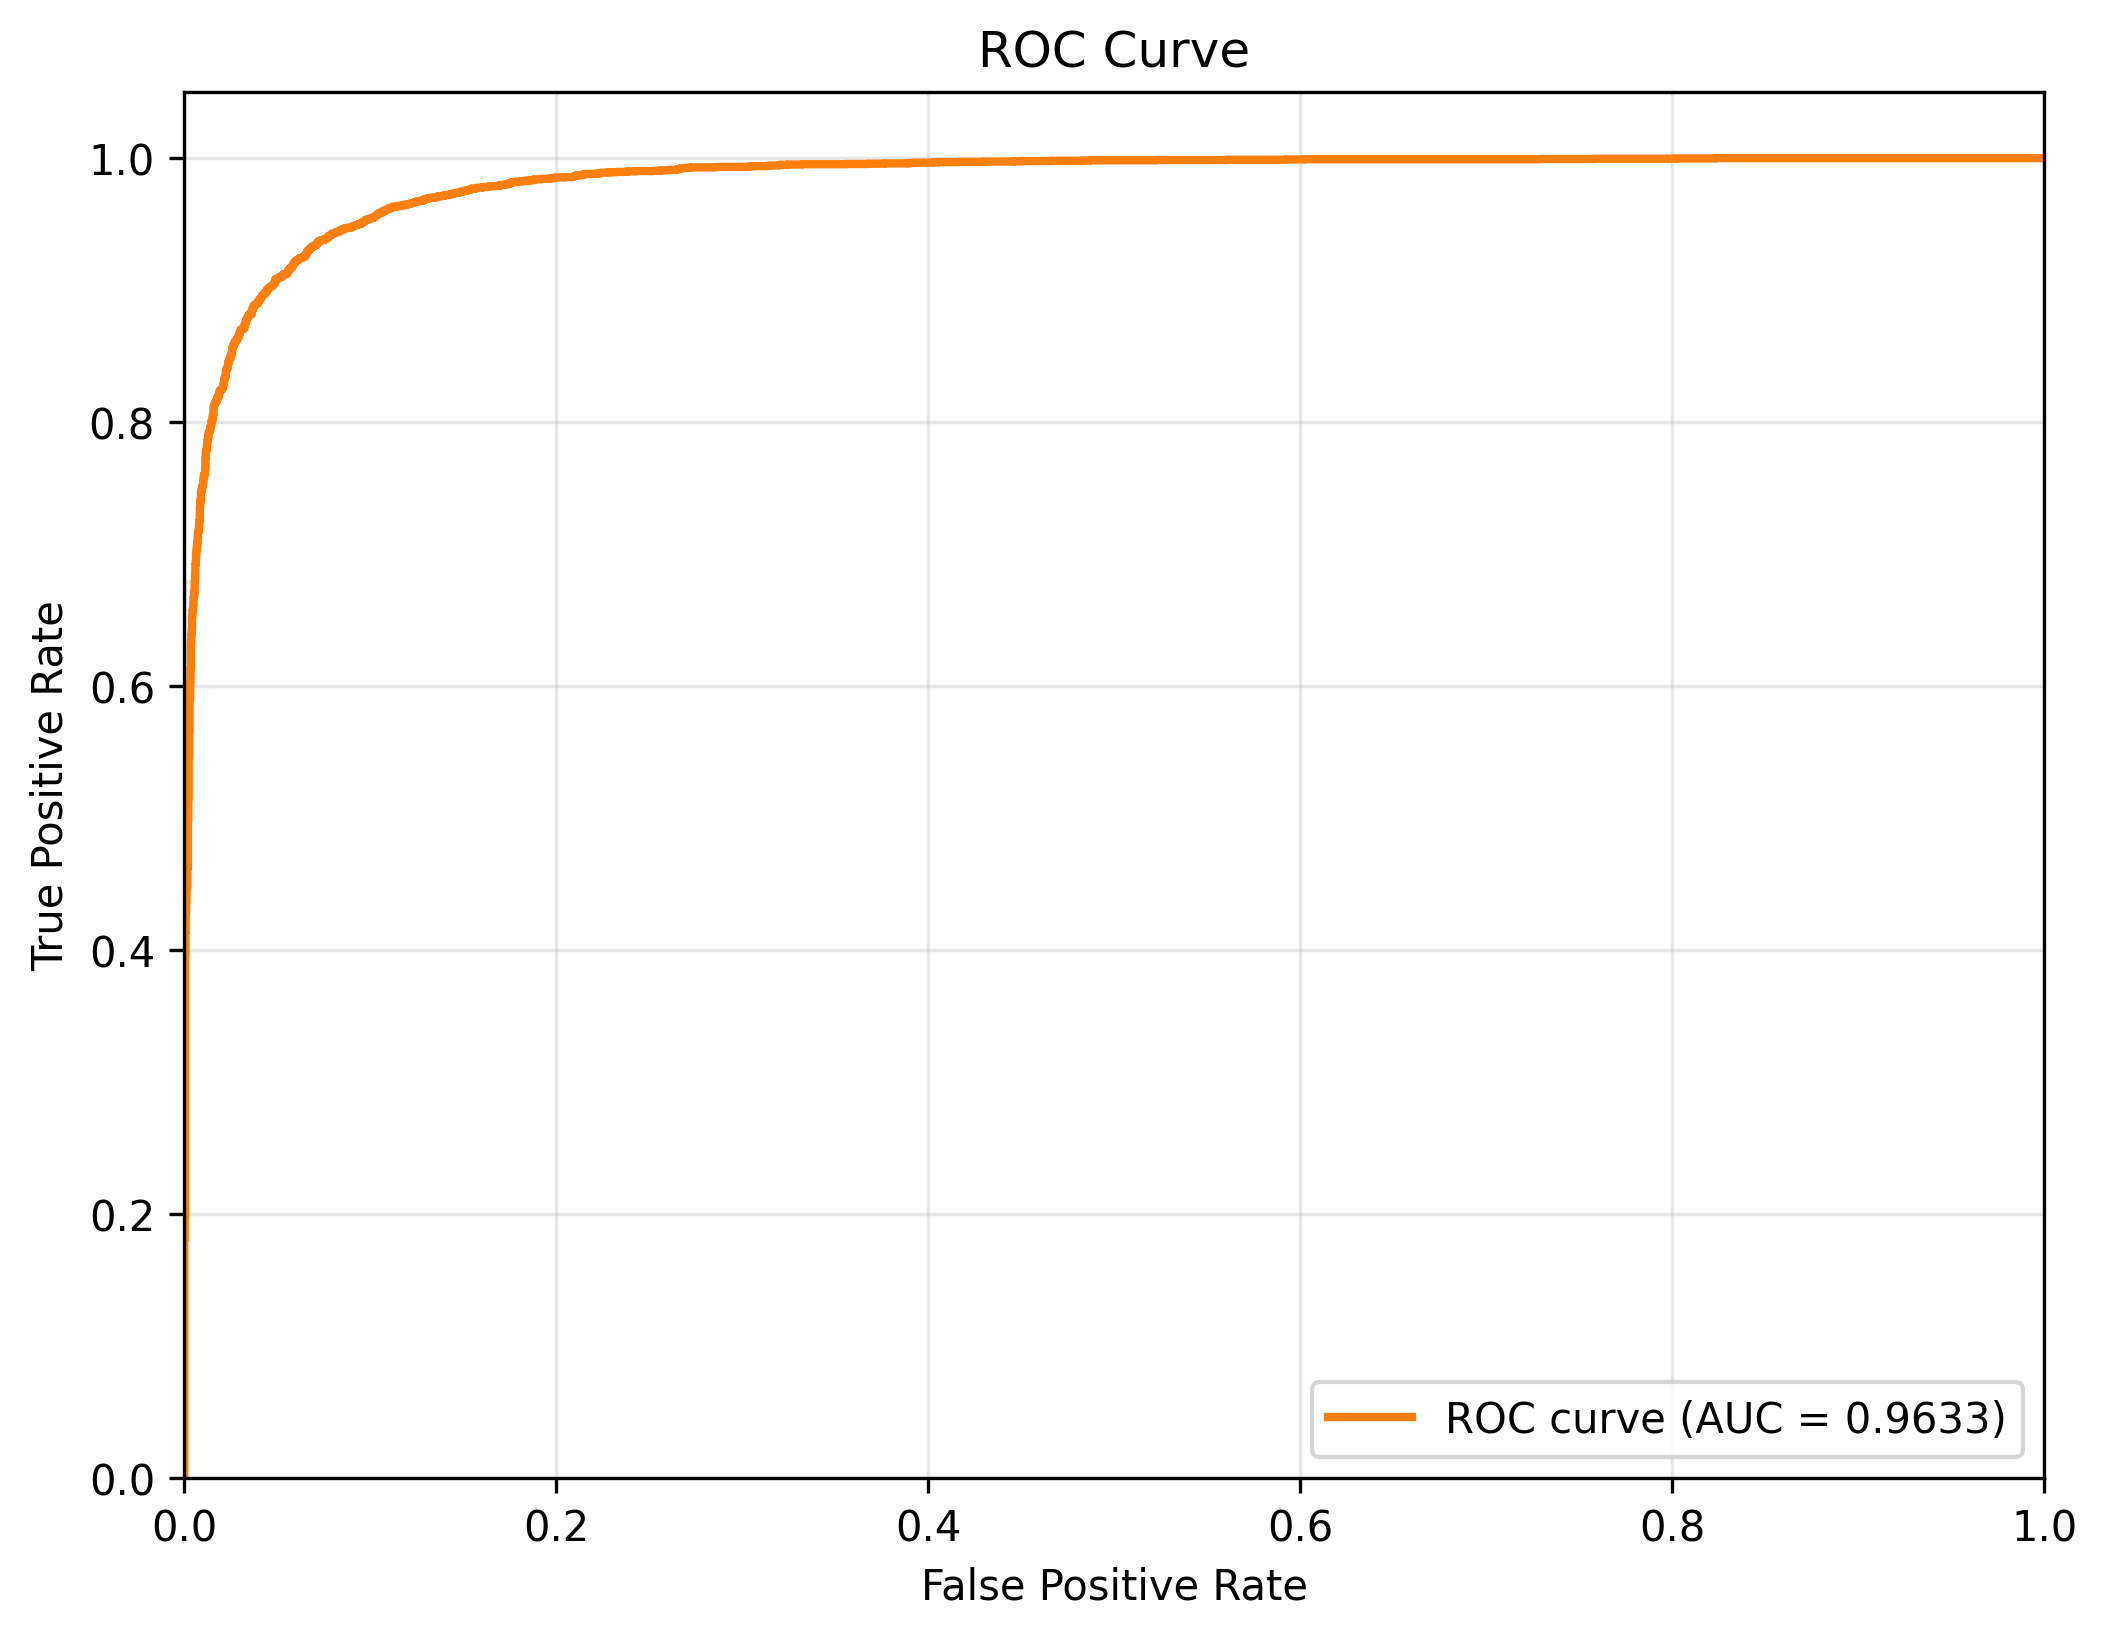
\includegraphics[width=.45\textwidth]{figures/outputs_stage3_run_20251030_081127_01_roc_curve.png}
  \caption{ROC curves for Stage~1 (left) and an expert model (right, EfficientNetV2) on combined validation.}
  \label{fig:roc_baselines}
\end{figure}
\FloatBarrier

\subsection{Per-Dataset Performance Analysis}

While aggregate metrics on the combined validation split provide a high\hyp level view of system performance, per\hyp dataset breakdowns reveal important differences in detection difficulty and model behavior across manipulation sources. We analyze Stage~1 and Stage~2 performance on four constituent datasets: CelebDF\hyp v2, FaceForensics++, DFDC, and DeeperForensics\hyp 1.0.

\subsubsection{CelebDF-v2 Characteristics}
CelebDF\hyp v2 comprises celebrity face swaps with high visual quality and controlled recording conditions. Per\hyp dataset Stage~1 results show that the lightweight filter performs very strongly on this dataset (high AUC and low FNR; Table~\ref{tab:stage1_per_dataset}), whereas the Stage~2 baseline at threshold 0.70 attains only moderate AUC (about \num{0.77}) and relatively high FNR (\num{0.38}; Table~\ref{tab:stage2_per_dataset}). This reflects CelebDF\hyp v2's design philosophy: fakes are intentionally subtle and can evade simple cues, making naive single\hyp threshold operation unacceptable and motivating cascade escalation and threshold tuning. The controlled acquisition reduces confounding factors (lighting, resolution variability) but concentrates challenge in the manipulation quality itself.

\subsubsection{FaceForensics++ Characteristics}
FaceForensics++ includes diverse manipulation methods (Deepfakes, Face2Face, FaceSwap, NeuralTextures) with varying levels of realism. Stage~1 achieves strong performance on this dataset (high AUC and F1; Table~\ref{tab:stage1_per_dataset}), suggesting that MobileNetV4 captures common artifacts across multiple generation methods when trained on combined data. However, Stage~2's performance at threshold 0.70 (AUC~\num{0.80}, FNR~\num{0.54}; Table~\ref{tab:stage2_per_dataset}) reveals that fixed thresholds are suboptimal---the high FNR stems from conservative threshold choice rather than fundamental model weakness. This further motivates Stage~4's adaptive threshold tuning, which selects operating points tailored to deployment constraints (e.g., FNR budget) rather than arbitrary cutoffs.

\subsubsection{DFDC (Deepfake Detection Challenge)}
DFDC represents highly heterogeneous data: diverse actors, recording devices, compression levels, and manipulation techniques. Stage~1 maintains strong per\hyp dataset metrics (Table~\ref{tab:stage1_per_dataset}), while Stage~2 at threshold 0.70 achieves AUC~\num{0.90} with a non\hyp trivial FNR (\num{0.16}; Table~\ref{tab:stage2_per_dataset}). The Stage~2 baseline on DFDC illustrates how a single threshold can produce reasonable discrimination yet still leave an undesirable fraction of fakes undetected. Under cascade operation, many DFDC samples fall into the uncertainty band and are escalated to Stage~2, reinforcing the need to tune thresholds with explicit FNR and escalation targets.

\subsubsection{DeeperForensics-1.0 Characteristics}
DeeperForensics\hyp 1.0 emphasizes robustness to perturbations (compression, blur, noise) and includes high\hyp quality fakes with temporal consistency. Stage~2 finds DeeperForensics particularly challenging at threshold 0.70: AUC remains moderate (\num{0.86}), but FNR is extremely high (\num{0.67}) and recall low (\num{0.33}; Table~\ref{tab:stage2_per_dataset}). The conservative threshold severely limits recall; this is precisely the scenario where cascade threshold tuning (Stage~4) provides value by lowering $\tau_{low}$ to escalate more borderline cases and shifting the operating point toward lower FNR. DeeperForensics's emphasis on temporal consistency and robustness also highlights a limitation of our frame\hyp level approach---future work on temporal aggregation could improve performance on such datasets.

\subsubsection{Cross-Dataset Patterns}
Comparing per\hyp dataset results reveals systematic patterns:
\begin{itemize}[leftmargin=*,itemsep=2pt,parsep=0pt]
  \item \textbf{Dataset difficulty correlates with heterogeneity.} Controlled datasets (CelebDF\hyp v2, FF++) yield high absolute performance but can still challenge detectors through subtle manipulation quality. Heterogeneous datasets (DFDC, DeeperForensics) exhibit lower AUC and higher FNR at fixed thresholds due to within\hyp dataset variation (recording conditions, quality, manipulation diversity).

  \item \textbf{Stage~1 vs.\ Stage~2 trade-offs vary by dataset.} On CelebDF\hyp v2 and FF++, Stage~1's simplicity suffices for many samples, with Stage~2 providing additional capacity primarily for ambiguous cases. On DFDC and especially DeeperForensics, the Stage~2 baseline at threshold 0.70 exposes how sensitive FNR is to threshold choice, and why a cascaded scheme with tuned thresholds is preferable to a single fixed cut\hyp off.

  \item \textbf{Fixed thresholds are suboptimal across datasets.} The threshold 0.70 used in Table~\ref{tab:stage2_per_dataset} yields markedly different operating points across datasets (FNR ranges from \num{0.16} to \num{0.67}), underscoring the need for per\hyp dataset or per\hyp deployment calibration. Our cascade threshold tuning (Stage~4) addresses this by selecting $(\tau_{low}, \tau_{high})$ pairs that meet system\hyp level constraints (e.g., target FNR $<$ 1\%) rather than dataset\hyp specific cutoffs.
\end{itemize}

These per\hyp dataset insights inform deployment strategy: for applications prioritizing recall (e.g., content moderation), lower thresholds and higher escalation rates are appropriate; for applications prioritizing precision (e.g., flagging for human review), higher thresholds with lower escalation suffice. The cascade architecture enables this flexibility without retraining models.

\subsection{Meta-Model (Stage 3) Analysis}
Stage~3 trains a LightGBM meta\hyp model on K\hyp fold out\hyp of\hyp fold features from the Stage~2 experts (EfficientNetV2 and optional GenConViT). In our current runs, the meta\hyp model achieves validation performance similar to, but on average slightly worse than, the strongest single expert (Table~\ref{tab:stage2_stage3}). Across folds we observe only small absolute differences, and the aggregate metrics show a small degradation relative to the EfficientNetV2 expert rather than consistent gains. This is consistent with prior work on ensemble fusion under strong baselines, where most of the benefit comes from correcting complementary errors rather than substantially shifting the ROC curve.

Given these modest deltas and the added complexity of maintaining separate meta\hyp model artifacts, our primary cascade results focus on a two\hyp stage configuration in which Stage~2 uses the best expert (EfficientNetV2) and Stage~3 is treated as an optional enhancement. The meta\hyp model remains valuable as an analysis tool: it confirms that expert features are highly informative and that there is limited residual complementarity to exploit under our current training mix. Future work could revisit this component with more diverse experts (e.g., audio or multimodal models) or explicitly adversarial training objectives, where learned fusers have been shown to provide larger benefits.

\begin{table}[h]
  \centering
  \caption{Stage~2 expert vs.\ Stage~3 meta-model on combined validation. Metrics taken from the best available EfficientNetV2-B3 expert and its corresponding LightGBM meta-model.}
  \label{tab:stage2_stage3}
  {\small
  \begin{tabular}{lccc}
    \toprule
    Model & AUC & F1 & FNR \\
    \midrule
    Stage~2 EfficientNetV2-B3 expert & 0.9633 & 0.8930 & 0.0943 \\
    Stage~3 LightGBM meta-model      & 0.9610 & 0.8869 & 0.1067 \\
    \bottomrule
  \end{tabular}}
\end{table}
\FloatBarrier

\begin{figure}[h]
  \centering
  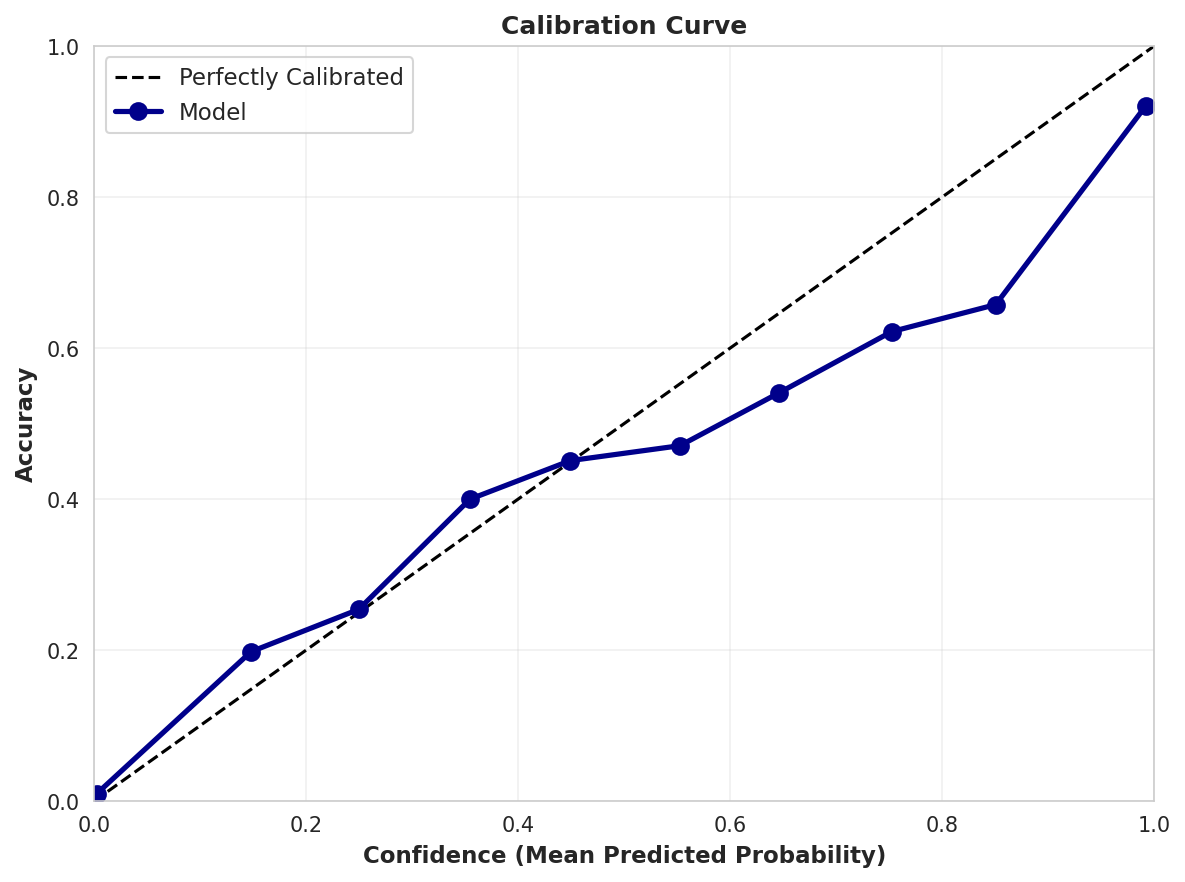
\includegraphics[width=.45\textwidth]{figures/outputs_stage1_run_20251023_034316_03_calibration.png}\hfill
  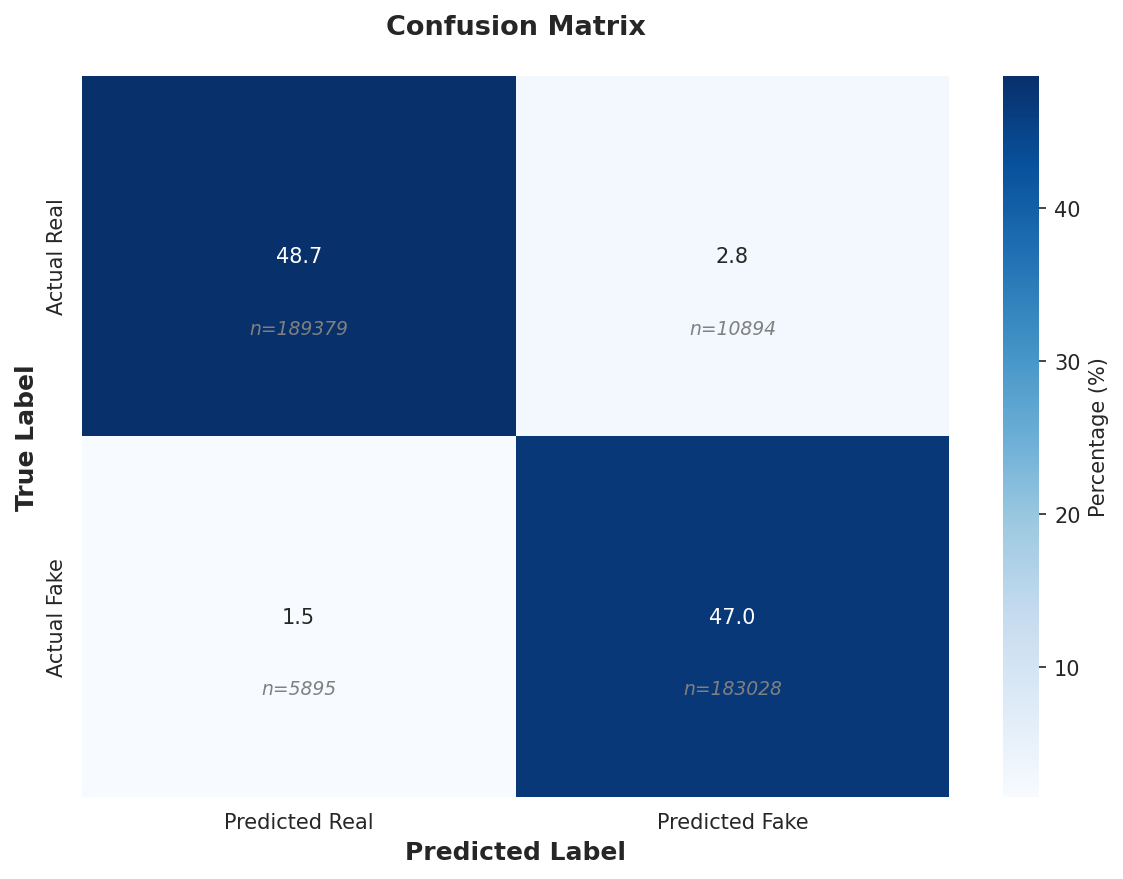
\includegraphics[width=.45\textwidth]{figures/outputs_stage1_run_20251023_034316_confusion_matrix.png}
  \caption{Stage~1 calibration (left) and confusion matrix (right).}
  \label{fig:stage1_calib_conf}
\end{figure}
\FloatBarrier

\begin{figure}[h]
  \centering
  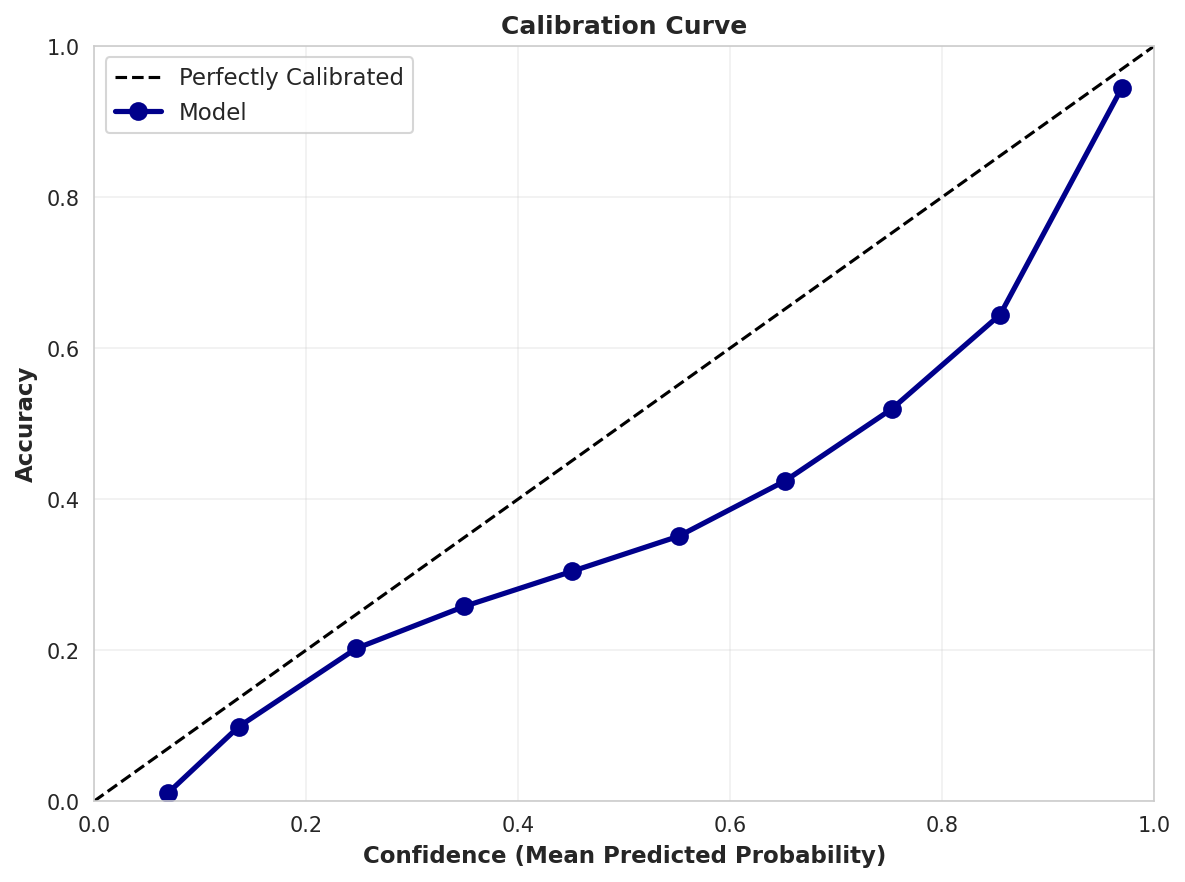
\includegraphics[width=.45\textwidth]{figures/outputs_stage3_run_20251030_081127_03_calibration.png}\hfill
  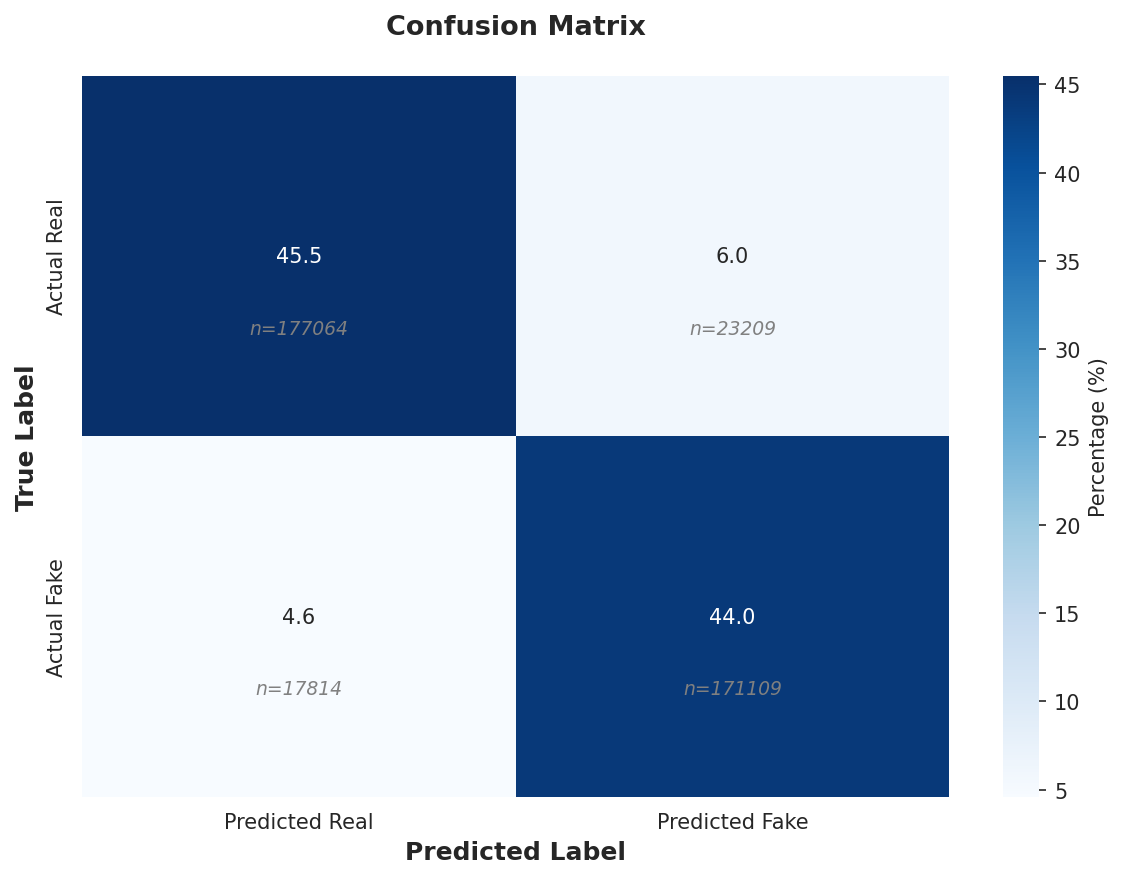
\includegraphics[width=.45\textwidth]{figures/outputs_stage3_run_20251030_081127_confusion_matrix.png}
  \caption{Stage~2 calibration (left) and confusion matrix (right).}
  \label{fig:stage2_calib_conf}
\end{figure}
\FloatBarrier

\subsection{Cascade Threshold Tuning}

\begin{table}[h]
  \centering
  \caption{Best cascade configurations (validation). Low/high thresholds, metrics, and escalation rate.}
  \label{tab:cascade_best}
  {\small
  \begin{tabular}{cccccc}
    \toprule
    Low & High & AUC & F1 & FNR & Escalation \\
    \midrule
    0.05 & 0.55 & \num{0.9941} & \num{0.9654} & \num{0.0060} & \num{0.0116} \\
    0.03 & 0.55 & \num{0.9941} & \num{0.9644} & \num{0.0054} & \num{0.0150} \\
    \bottomrule
  \end{tabular}}
\end{table}

The two configurations in Table~\ref{tab:cascade_best} illustrate the core trade\hyp off. Tightening $\tau\_{low}$ from $0.05$ to $0.03$ reduces the false negative rate from \num{0.0060} to \num{0.0054}, but increases the Stage~2 escalation rate from \num{1.16}\% to \num{1.50}\%. In terms of the Stage~1 leakage rate $\pi\_{\mathrm{leak}}$, the lower threshold configuration accepts fewer borderline fakes at Stage~1 and delegates more samples to the expert; this behaviour is desirable in high\hyp risk deployments where missed fakes are costly, and the incremental compute is modest given the low baseline escalation.

We adopt probability calibration (temperature scaling) on Stage~2 prior to threshold selection when transferring thresholds across datasets, following \cite{guo2017calibration}; under distribution shift, calibration effects can vary and should be reported with care \cite{minderer2021revisiting}. In our experiments, calibration slightly improves alignment between predicted probabilities and empirical frequencies on the combined validation set and stabilises the Pareto frontier of $(\mathrm{FNR}, \pi\_2)$ across nearby operating points, but does not fully close the gap on Deepfake\hyp Eval\hyp 2024.

\begin{figure}[h]
  \centering
  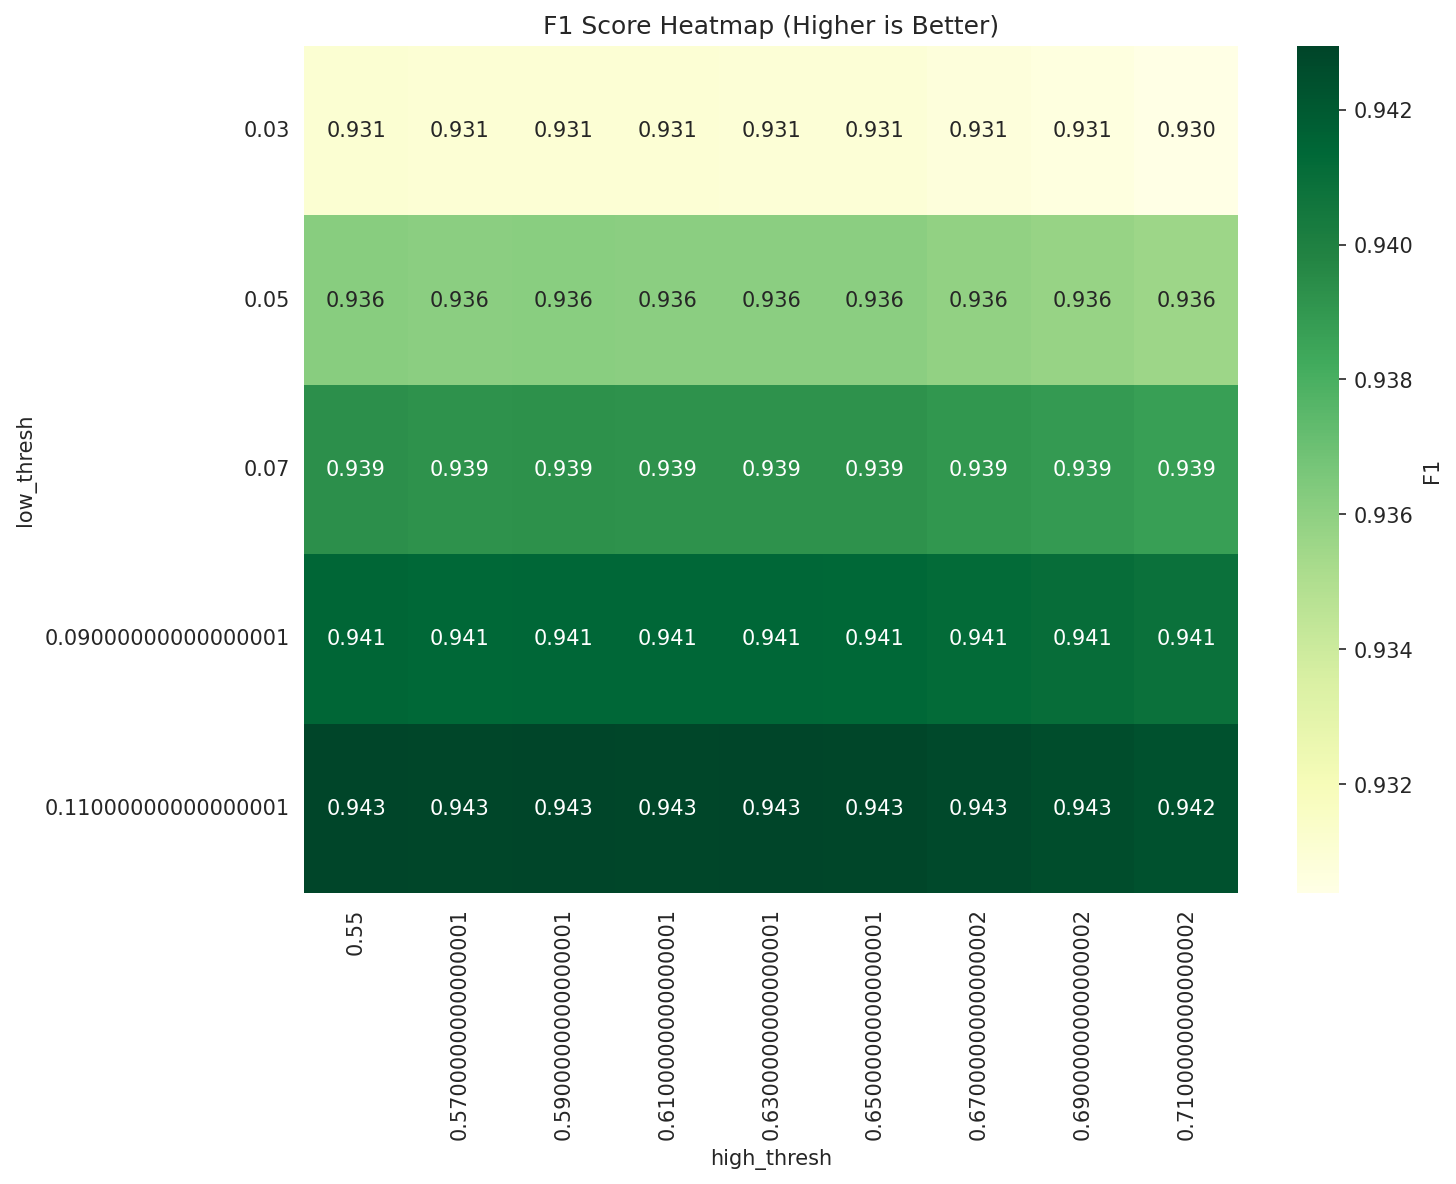
\includegraphics[width=.32\textwidth]{figures/outputs_stage4_run_20251031_075851_heatmap_f1.png}\hfill
  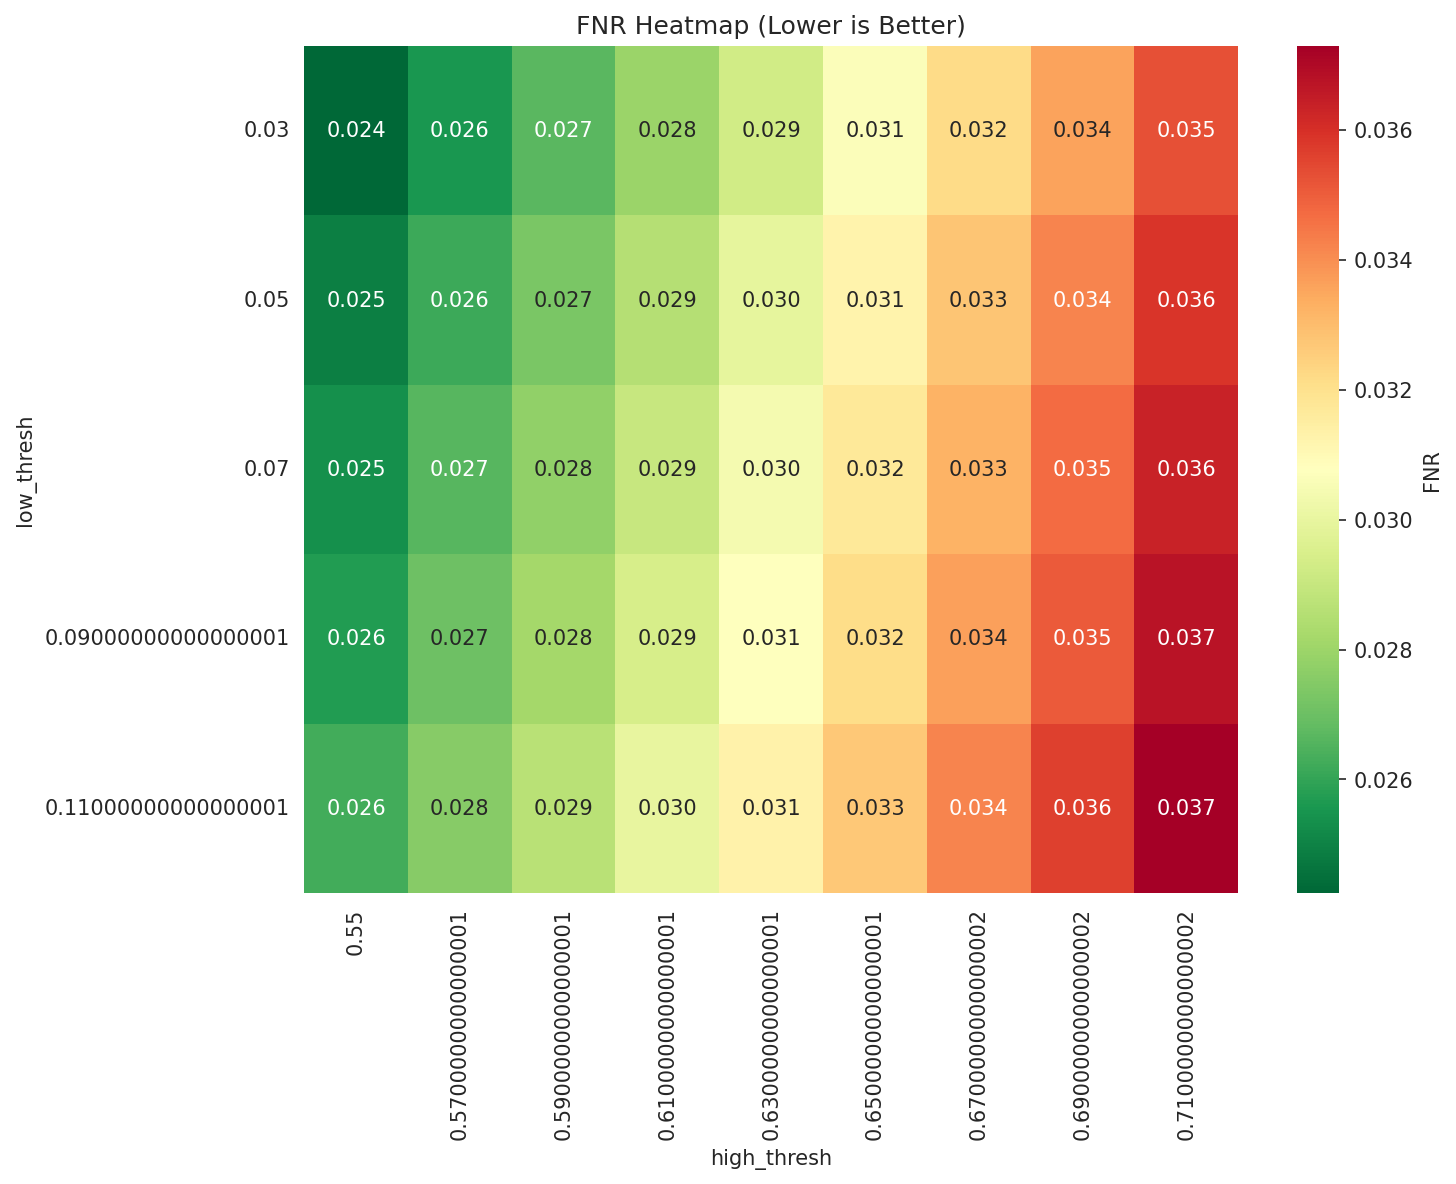
\includegraphics[width=.32\textwidth]{figures/outputs_stage4_run_20251031_075851_heatmap_fnr.png}\hfill
  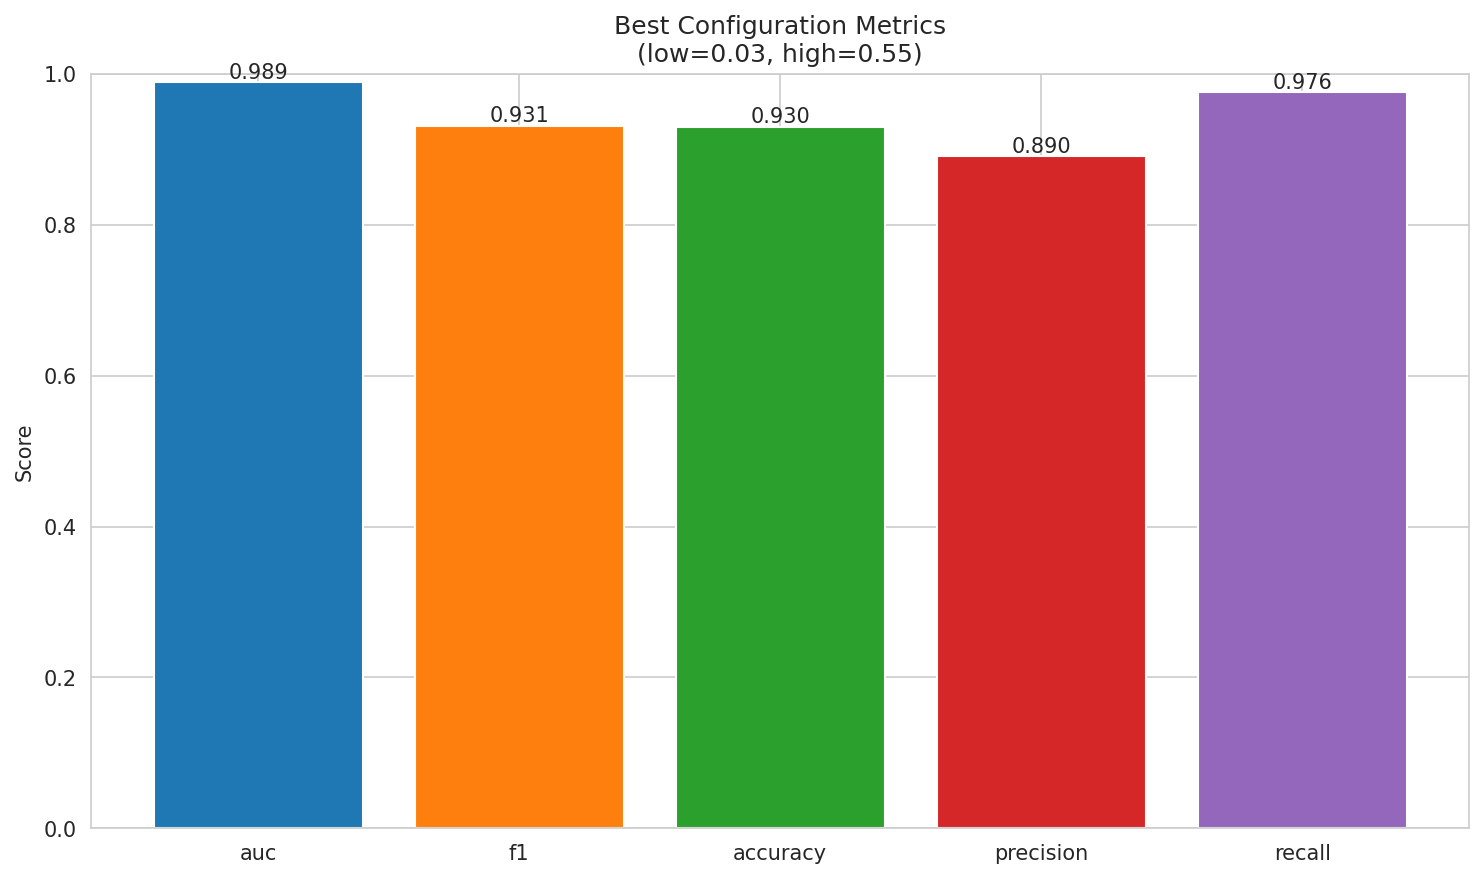
\includegraphics[width=.32\textwidth]{figures/outputs_stage4_run_20251031_075851_best_config_metrics.png}
  \caption{Cascade threshold tuning heatmaps and best configuration metrics (example run).}
  \label{fig:cascade_heatmaps}
\end{figure}
\FloatBarrier

\subsection{Cross-Dataset Evaluation (Deepfake-Eval-2024)}
% The Deepfake-Eval-2024 calibrated and Stage2-only tables are included in the auto tables above.

On Deepfake\-Eval\-2024, the calibrated cascade performs substantially worse than on in\-distribution validation (Table~\ref{tab:deepeval_calibrated}): F1 falls below \num{0.30} on both validation and test splits, and FNR remains high ($\approx$\num{0.73}--\num{0.79}) even though only around half of the samples are escalated to Stage~2 (Stage~2 rate $\approx$\num{0.51}). This gap aligns with known failure modes on in\hyp the\hyp wild media~\cite{wilddeepfake2021,pei2024deepfakesurvey,deepeval2024}: (i) preprocessing mismatch (resolution, compression, face crops) between training data and social\hyp media distribution; (ii) missing or underrepresented generation methods and post\-processing pipelines during training; and (iii) detectors inadvertently learning dataset\-specific artifacts that do not transfer.

A Stage~2\-only setting (Table~\ref{tab:deepeval_stage2only}) serves as a crude upper bound when the expert handles nearly all samples. It attains higher F1 on the test split (F1~\num{0.60}, FNR~\num{0.15}) but at the cost of extremely high false positive rates (FPR~$\approx$\num{0.87}--\num{0.92}) and near\hyp maximal Stage~2 usage (Stage~2 rate~$\ge$\num{0.97}). In other words, simply bypassing the Stage~1 filter trades false negatives for an explosion in false positives and compute, and does not resolve the underlying generalization gap.

Qualitatively, we observe that failures on Deepfake\hyp Eval\hyp 2024 often concentrate on clips with heavy recompression, strong editing, or atypical framing (e.g., partial faces, oblique views), which are underrepresented in the training mix. The cascade remains conservative---escalation rates increase relative to in\hyp distribution validation as more samples fall into the ambiguous band---but the expert itself is less calibrated, leading to higher residual FNR even after temperature scaling. Improving robustness and calibration on truly in\hyp the\hyp wild data therefore requires more than simple threshold transfer.

Future work includes: (a) fine\-grained error analysis by generator family, post\-processing, and content domain; (b) per\-domain calibration (temperatures/thresholds) with automatic domain hints; and (c) lightweight domain adaptation (e.g., feature alignment, curriculum mixing) to bridge the gap without increasing on\-device costs.

% Auto-generated robustness figures
\begin{figure}[h]
  \centering
  % Use paths relative to paper/ directory for portability; break lines to avoid overflow
  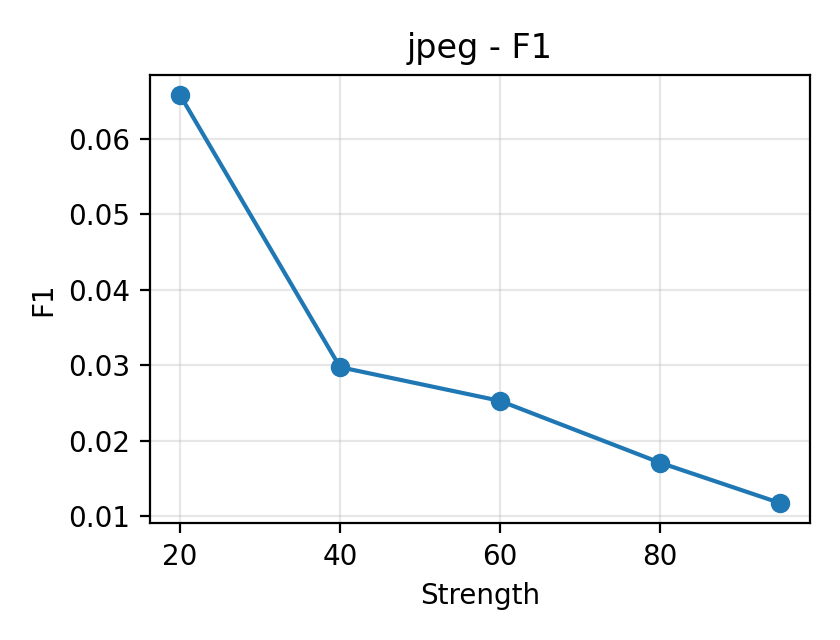
\includegraphics[width=.32\textwidth]{figures/figures_outputs_stage5_robustness_jpeg_f1.png}% jpeg
  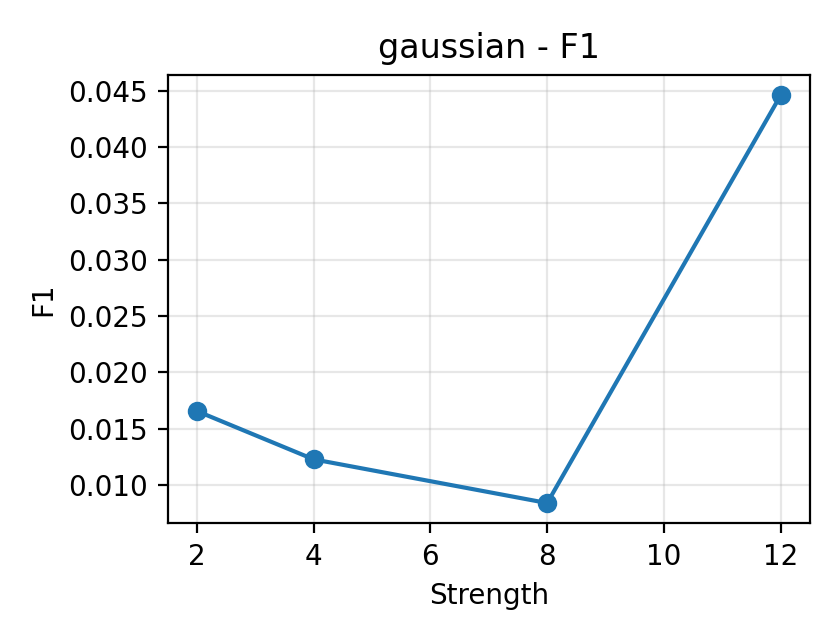
\includegraphics[width=.32\textwidth]{figures/figures_outputs_stage5_robustness_gaussian_f1.png}% gaussian
  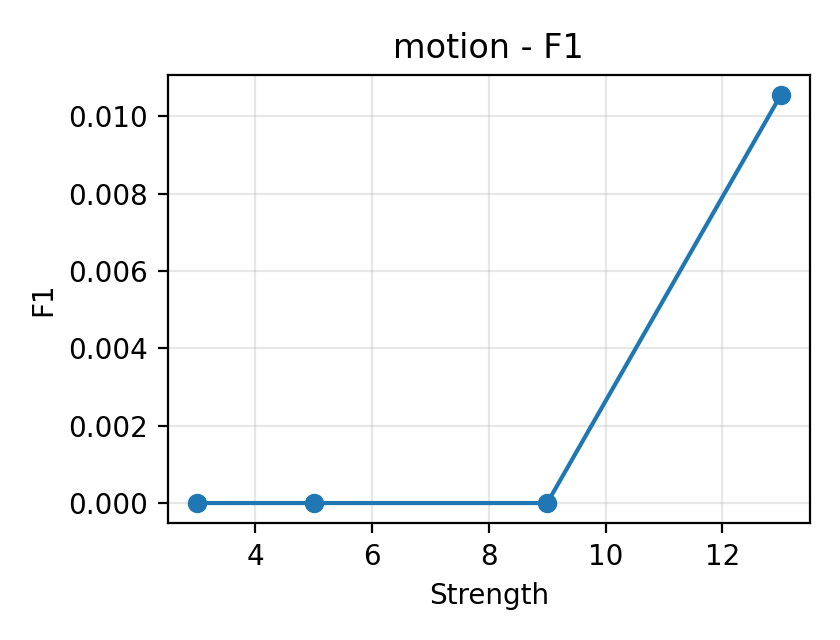
\includegraphics[width=.32\textwidth]{figures/figures_outputs_stage5_robustness_motion_f1.png}% motion\\
  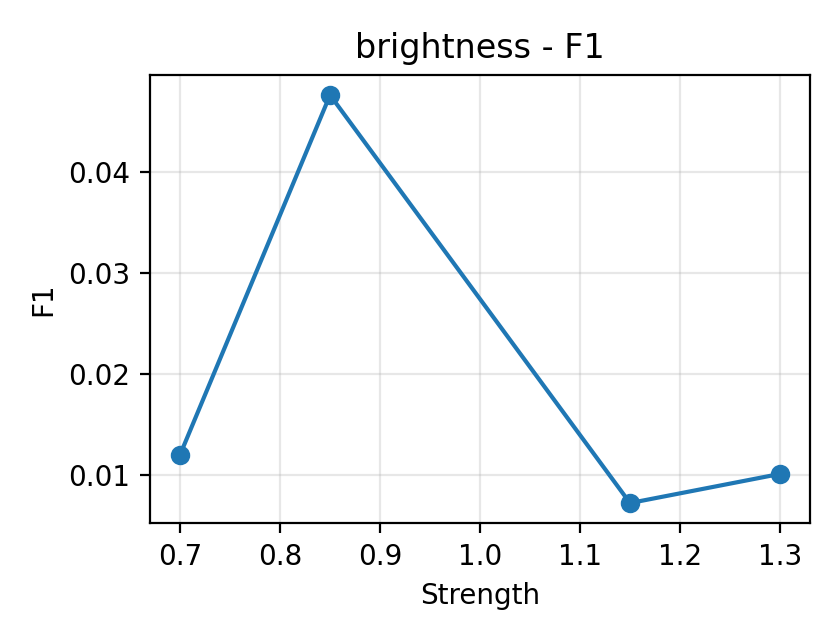
\includegraphics[width=.32\textwidth]{figures/figures_outputs_stage5_robustness_brightness_f1.png}% brightness
  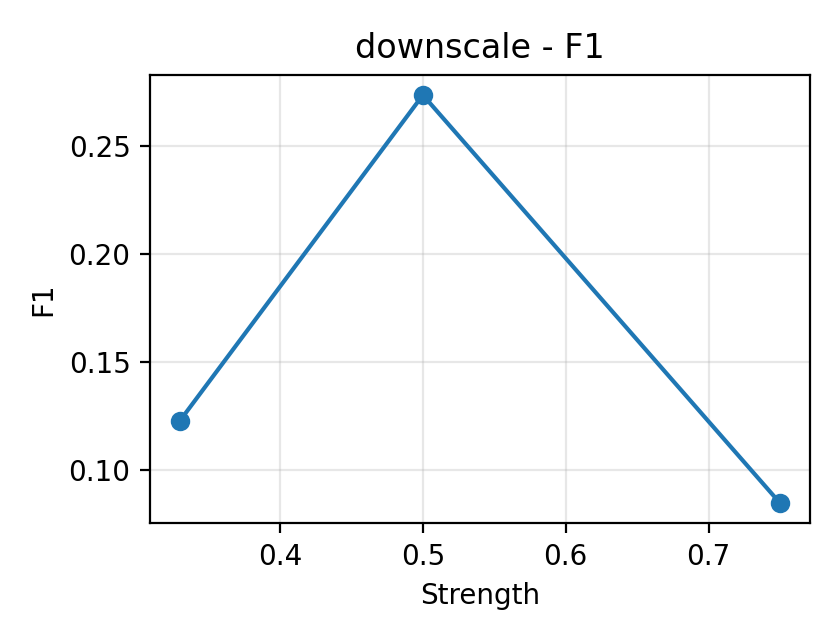
\includegraphics[width=.32\textwidth]{figures/figures_outputs_stage5_robustness_downscale_f1.png}% downscale
  \caption{Robustness: metric curves under common perturbations.}
  \label{fig:robustness_curves}
\end{figure}

\FloatBarrier

\subsection{Routing Strategies: Confidence vs. Entropy vs. Margin}
We compare confidence\-based routing (ours) with entropy and margin alternatives (template deferred to future work) \cite{kaya2019shallowdeep}. Confidence routing offers direct control of the escalation rate via $(\tau_{\mathrm{low}},\tau_{\mathrm{high}})$ and pairs well with calibration; entropy and margin can be emulated within the same framework. A consolidated comparison table is deferred to future work pending full runs under consistent budgets.

\subsection{Robustness to Common Perturbations}
We evaluate the tuned cascade under four perturbation types (JPEG compression, Gaussian noise, motion blur, and brightness/contrast) using the same combined validation manifest. Figure~\ref{fig:robustness_curves} plots F1 vs.\ perturbation strength, while Table~\ref{tab:robustness_table} aggregates F1/Acc/FNR/Stage~2 rate for representative levels, and Figure~\ref{fig:robustness_tradeoff} shows FNR vs.\ Stage~2 rate under threshold sweeps. Although these experiments are preliminary and would benefit from larger samples, several consistent patterns emerge:
\begin{itemize}[leftmargin=*]
  \item \textbf{JPEG compression.} As JPEG quality decreases from 95 to 20, F1 and accuracy fluctuate but do not collapse; in some settings, moderate compression slightly \emph{improves} F1 and lowers FNR (Table~\ref{tab:robustness_table}). This is consistent with frequency\hyp based analyses~\cite{durall2020watch,qian2020thinkingfrequency}: compression can accentuate artifacts that detectors rely on. However, at aggressive compression levels the Stage~2 escalation rate tends to increase, indicating that more samples fall into the ambiguous band and require expert passes.
  \item \textbf{Gaussian noise.} Increasing noise (e.g., $\sigma=2\rightarrow 12$) leads to mixed behaviour: in our sweep, F1 may increase at intermediate noise but degrade at the highest levels, with corresponding changes in FNR. A plausible explanation is that strong noise perturbs real textures more than fake cues under the current thresholds, effectively acting as a domain shift; per\hyp family calibration (Section~\ref{tab:robustness_table}) and larger runs are needed to stabilise these trends.
  \item \textbf{Motion blur.} For kernel sizes in the range tested (3--13), F1 and FNR change gradually rather than catastrophically, suggesting that the cascade retains partial robustness to modest blur. As with JPEG, higher blur tends to increase Stage~2 usage because more inputs are routed out of the high\hyp confidence band at Stage~1.
  \item \textbf{Brightness/contrast.} Moderate brightness changes (e.g., 0.7--1.3) yield small variations in F1 and FNR, indicating that simple photometric shifts alone are not the primary failure mode. Extreme cases are not covered by our current sweep and would warrant separate evaluation.
\end{itemize}
Overall, these results motivate per\hyp family threshold/temperature calibration and consistent reporting of Stage~2 escalation rates to quantify efficiency\hyp robustness trade\hyp offs. Prior analyses suggest frequency artifacts from generative up\hyp sampling are informative \cite{durall2020watch}, and adaptive frequency filtering can be beneficial~\cite{qian2020thinkingfrequency}. JPEG and noise may accentuate some cues at certain thresholds; a per\hyp family calibration protocol is therefore appropriate. Beyond natural perturbations, adversarial attacks (e.g., CW, PGD) can severely degrade detector performance if unaccounted for \cite{carlini2017towards}; reporting calibrated thresholds and escalation rates helps bound risk under operational budgets.

\paragraph{Temporal segmentation and partial forgeries.} Beyond video\hyp level decisions, frame\hyp level segmentation of forged segments has been explored to handle partial manipulations \cite{undercover2023}. Our two\hyp stage architecture is compatible with such post\hyp processing: Stage~1 can pre\hyp filter frames and Stage~2 can refine segment boundaries under a budget.

\begin{table}[h]
  \centering
  \caption{Robustness summary by perturbation and level.}\label{tab:robustness_table}
  \begin{tabular}{lcrrrr}\toprule
 Perturbation & Level & F1 & Acc & FNR & S2 Rate \\ \midrule
  brightness & 0.7 & 0.0120 & 0.8360 & 0.9796 & 0.7490 \\ 
  brightness & 0.85 & 0.0476 & 0.8400 & 0.9184 & 0.7000 \\ 
  brightness & 1.15 & 0.0073 & 0.7270 & 0.9796 & 0.2440 \\ 
  brightness & 1.3 & 0.0102 & 0.8050 & 0.9796 & 0.1730 \\ 
  gaussian & 12.0 & 0.0446 & 0.3150 & 0.6735 & 0.4850 \\ 
  gaussian & 2.0 & 0.0166 & 0.5250 & 0.9184 & 0.4190 \\ 
  gaussian & 4.0 & 0.0123 & 0.6780 & 0.9592 & 0.2720 \\ 
  gaussian & 8.0 & 0.0084 & 0.5270 & 0.9592 & 0.4100 \\ 
  jpeg & 20.0 & 0.0658 & 0.0350 & 0.3061 & 0.0520 \\ 
  jpeg & 40.0 & 0.0298 & 0.0870 & 0.7143 & 0.3590 \\ 
  jpeg & 60.0 & 0.0253 & 0.1520 & 0.7755 & 0.7320 \\ 
  jpeg & 80.0 & 0.0171 & 0.4250 & 0.8980 & 0.6450 \\ 
  jpeg & 95.0 & 0.0117 & 0.4950 & 0.9388 & 0.5810 \\ 
  motion & 13.0 & 0.0106 & 0.6250 & 0.9592 & 0.3760 \\ 
  motion & 3.0 & 0.0000 & 0.0890 & 1.0000 & 0.2110 \\ 
  motion & 5.0 & 0.0000 & 0.0290 & 1.0000 & 0.1900 \\ 
  motion & 9.0 & 0.0000 & 0.8330 & 1.0000 & 0.1670 \\ 
  \bottomrule\end{tabular}\end{table}

\FloatBarrier

% Robustness trade-off figures (FNR vs Stage-2 rate under threshold sweeps)
% Note: These figures are generated from outputs/stage5/robustness using the
% robustness_threshold_sweep utility. To regenerate, run:
%   python -m src.tools.robustness_threshold_sweep [args...]
%
% Currently disabled: fnr_vs_s2 plots are not available (outputs/ directory is gitignored).
% To re-enable, regenerate the plots and uncomment the figure below.
%
% \begin{figure}[h]
%   \centering
%   \includegraphics[width=.32\textwidth]{../outputs/stage5/robustness/fnr_vs_s2_jpeg_20.0.png}\hfill
%   \includegraphics[width=.32\textwidth]{../outputs/stage5/robustness/fnr_vs_s2_jpeg_95.0.png}\hfill
%   \includegraphics[width=.32\textwidth]{../outputs/stage5/robustness/fnr_vs_s2_gaussian_12.0.png}
%   \caption{Representative FNR vs Stage-2 escalation rate trade-off curves under threshold sweeps. Left: JPEG quality 20 (heavy compression); middle: JPEG quality 95 (light compression); right: Gaussian noise with $\sigma=12$.}
%   \label{fig:robustness_tradeoff}
% \end{figure}

\FloatBarrier

\subsection{Error Analysis and Failure Mode Taxonomy}

Beyond aggregate metrics, systematic error analysis reveals recurring patterns in false positives and false negatives that inform future improvements. Using qualitative inspection of diagnostic plots and per\hyp sample predictions across Stage~1 and Stage~2, we observe that:
\begin{itemize}[leftmargin=*,itemsep=2pt,parsep=0pt]
  \item \textbf{False positives} are dominated by heavily compressed or low\hyp quality real videos, unusual lighting and makeup, and challenging viewpoints or occlusions. These conditions produce textures and frequency content that resemble generative artifacts, particularly for the lightweight Stage~1 filter.
  \item \textbf{False negatives} arise from high\hyp quality fakes (including newer GAN and diffusion families), partial manipulations confined to small facial regions, and fakes that have been post\hyp processed to closely match surrounding real content. Such cases are common on Deepfake\hyp Eval\hyp 2024 and contribute to its high FNR.
\end{itemize}
Mitigations include stronger data augmentation (compression, occlusions, photometric changes), hard example mining (already used in Stage~2), and domain adaptation techniques (e.g., DA\-BN~\cite{li2021dabn}, unsupervised feature alignment) to better cover new generators. Temporal aggregation and multi\hyp frame consistency checks provide complementary signals beyond per\hyp frame classification, especially for partial or temporally localized manipulations.

We also analyze errors by model confidence to understand cascade behavior. Low\hyp confidence predictions tend to correspond to heavily degraded real videos where even the expert struggles; mid\hyp confidence cases mix FP and FN and benefit most from escalation; and high\hyp confidence errors, though rare, typically reflect systematic blind spots tied to specific generators or post\hyp processing styles. The two\hyp threshold routing policy naturally separates these regimes: samples with $p < \tau_{low}$ or $p > \tau_{high}$ receive confident Stage~1 decisions, while those with $\tau_{low} \le p \le \tau_{high}$ are escalated. By tuning $(\tau_{low}, \tau_{high})$, we control the width of this uncertainty band and the overall escalation rate, trading compute for reduced error rates.

Finally, exported visual error panels provide concrete examples of the above patterns (compressed real videos and unusual lighting among FPs; high\hyp quality and post\hyp processed fakes among FNs). These artifacts form a basis for more systematic taxonomies by generator family, post\hyp processing type, and content domain in future work.

\subsection{On-device Results}
\label{sec:ondevice_results}

To validate that the cascade transfers correctly to mobile deployment, we evaluate the exported ONNX models on the \texttt{mobile\_eval} subset (152 images) using a Xiaomi~13 smartphone (Snapdragon~8~Gen~2). The results, summarised in Tables~\ref{tab:mobile_runtime_auto} and~\ref{tab:mobile_accuracy_auto}, demonstrate practical on\hyp device performance.

\paragraph{Key Findings.}
The on\hyp device cascade achieves 92.8\% accuracy with an FNR of 2.5\% and FPR of 12.5\%. The low FNR indicates that the conservative bias of the PC\hyp tuned cascade transfers to mobile: the system continues to prioritise catching deepfakes over minimising false alarms. The Stage~2 escalation rate on \texttt{mobile\_eval} is 7.2\%, higher than the 1.2\% observed on the combined validation set. This increase reflects distribution differences between the compact \texttt{mobile\_eval} subset and the larger PC validation manifest rather than platform\hyp specific degradation.

\paragraph{Latency.}
Average per\hyp image latency is approximately 180\,ms, comprising $\sim$3\,ms for preprocessing and $\sim$176\,ms for ONNX inference. This latency is roughly $2\times$ higher than the desktop CPU baseline (Table~\ref{tab:mobile_perf}), which is expected given mobile thermal and power constraints. For interactive single\hyp image detection, 180\,ms provides near\hyp instantaneous feedback; for batch processing, the system can analyse approximately 5--6 images per second.

\paragraph{Comparison with PC Results.}
Table~\ref{tab:pc_vs_mobile} compares key metrics between the desktop combined validation set and the mobile \texttt{mobile\_eval} subset. The cascade maintains low FNR on both platforms ($<$3\%), demonstrating that the threshold configuration ($\tau_\mathrm{low}=0.02$, $\tau_\mathrm{high}=0.98$) generalises across runtimes. The higher FPR and escalation rate on mobile primarily reflect the different sample composition of \texttt{mobile\_eval} rather than model export artefacts.

\begin{table}[h]
  \centering
  \caption{PC vs.\ mobile cascade comparison. PC metrics from combined validation; mobile metrics from \texttt{mobile\_eval} (152 images).}
  \label{tab:pc_vs_mobile}
  {\small
  \begin{tabular}{lcccc}
    \toprule
    Platform & Acc & FNR & FPR & Stage~2 Rate \\
    \midrule
    PC (combined val) & 0.97 & 0.006 & 0.03 & 0.012 \\
    Xiaomi~13 (mobile\_eval) & 0.93 & 0.025 & 0.125 & 0.072 \\
    \bottomrule
  \end{tabular}}
\end{table}

These results confirm that the two\hyp stage cascade is viable for privacy\hyp preserving, on\hyp device deepfake detection on consumer smartphones, with performance characteristics consistent with the desktop evaluation.

